\documentclass[tikz,border=8pt]{standalone}
% Shared look for every TikZ diagram. Load with \input{../../tools/tikz-style.tex}
\usepackage[T1]{fontenc}
\usepackage{lmodern}
\renewcommand{\sfdefault}{lmr}  % diagrams use the same serif as the text
\usetikzlibrary{arrows.meta, positioning, shapes.geometric, calc, fit, backgrounds}
\definecolor{cblue}{HTML}{4C78A8}
\definecolor{corange}{HTML}{F58518}
\definecolor{cgreen}{HTML}{54A24B}
\definecolor{cred}{HTML}{E45756}
\definecolor{cpurple}{HTML}{B279A2}
\definecolor{cgrey}{HTML}{6B6B6B}
\tikzset{
  every picture/.style={font=\sffamily, line width=1.2pt},
  box/.style={draw=#1, fill=#1!12, rounded corners=4pt, align=center, inner sep=7pt, minimum height=1.1cm},
  box/.default=cgrey,
  arrow/.style={-{Stealth[length=3mm]}, draw=cgrey, line width=1.4pt},
  title/.style={font=\sffamily\bfseries\Large},
  note/.style={font=\sffamily\small, text=cgrey, align=center},
}
\AtBeginDocument{\hyphenpenalty=10000 \exhyphenpenalty=10000}

\begin{document}
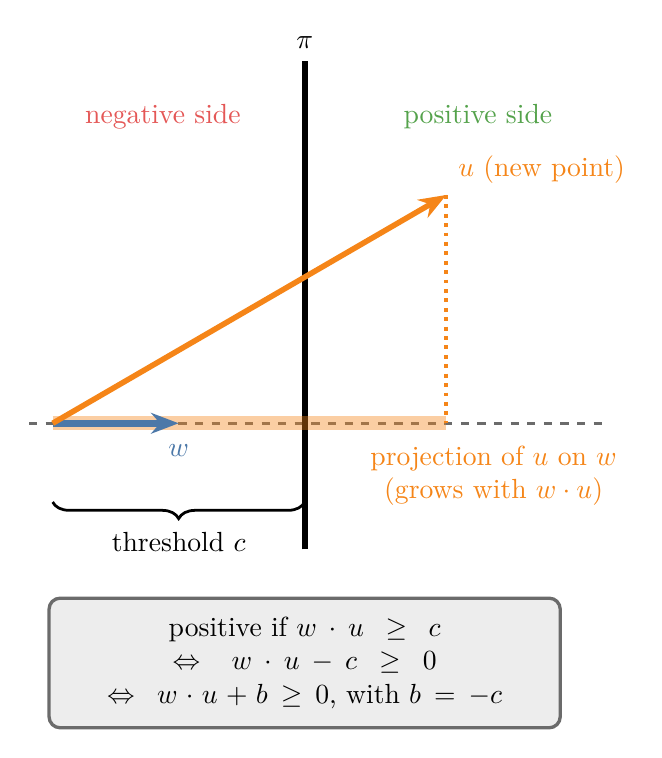
\begin{tikzpicture}
  \draw[cgrey, line width=1pt, dashed] (-0.3,0) -- (7,0);
  \draw[line width=2.2pt] (3.2,-1.6) -- (3.2,4.6) node[above] {$\pi$};
  \node[cred] at (1.4,3.9) {negative side};
  \node[cgreen] at (5.4,3.9) {positive side};
  \draw[line width=5pt, corange, opacity=0.4] (0,0) -- (5,0);
  \draw[-{Stealth[length=3.5mm]}, line width=2.4pt, cblue] (0,0) -- (1.6,0) node[below=3pt] {$w$};
  \draw[-{Stealth[length=3.5mm]}, line width=2pt, corange] (0,0) -- (5,2.9) node[above right] {$u$ (new point)};
  \draw[dotted, line width=1.4pt, corange] (5,2.9) -- (5,0);
  \node[corange, align=center, below] at (5.6,-0.15) {projection of $u$ on $w$\\(grows with $w \cdot u$)};
  \draw[decorate, decoration={brace, amplitude=6pt, mirror}, line width=1pt] (0,-1.0) -- (3.2,-1.0)
       node[midway, below=7pt] {threshold $c$};
  \node[box=cgrey, anchor=north, text width=6cm] at (3.2,-2.2) {positive if $w \cdot u \geq c$\\ $\Leftrightarrow\ w \cdot u - c \geq 0$\\ $\Leftrightarrow\ w \cdot u + b \geq 0$, with $b = -c$};
\end{tikzpicture}
\end{document}
